%
% 1dim.tex -- 
%
% (c) 2019 Prof Dr Andreas Mueller
%
\section{The one-dimensional problem}
\rhead{The one-dimensional case}
As a demonstration that the program sketched in the previous section
may actually be implemented, we consider the one dimensional problem
\[
u''(x)=f(x)
\]
on the interval $[0,1]$ with boundary conditions
\[
u(0)=a,\quad u(1)=b.
\]
The goal is to find the function $G(x,\xi)$.

THe solution of this problem usually is treated in the theory of
ordinary differential equations.
Here we would slightly modify the presentation in such a way
that it leads to $G$ and is more easily generalizable to 
multiple independent variables.

\subsection{Particular solution}
It is easy to find a particular solution, just take an antiderivative
of $f$ as in
\begin{align*}
u_p'(x)&=\int_0^xf(\xi)\,d\xi,
\\
u_p(x)&=\int_0^xu_p'(\eta)\,d\eta=\int_0^x\int_0^\eta f(\xi)\,d\xi\,d\eta.
\end{align*}
However, this solution does not satisfy the boundary conditions.
For this we have to add a suitable solution of the homogeneous
equation
\[
u_p''(x) + u_r''(x)=f(x)\quad\Rightarrow\quad u_r''(x)=0
\]
with boundary conditions
\begin{align*}
u_r(0)&=a-u_p(0)=a\\
u_r(1)&=b-u_p(1)=b-\int_0^1\int_0^\eta f(\xi)\,d\xi\,d\eta
\end{align*}

\subsection{The homogeneous problem}
The homogeneous problem
\[
u''(x)=0
\]
is even easier to solve.
The general solution is $Ax+B$, and the constants have to chosen
so that the boundary conditions hold, i.~e.
\begin{align*}
A\cdot 0+B&=a\qquad\Rightarrow&B&=a\\
A\cdot 1+B&=b\qquad\Rightarrow&A&=b-a
\end{align*}
which leads to $u(x)=(b-a)x+a=(1-x)a+xb$.

\subsection{General solution}
In the present example, $u_r$ is expected to take the boundary value
$b-\int_0^1\int_0^\eta f(\xi)\,d\xi\,d\eta$
für $x=1$, i.~e.
\[
u_r(x)=(1-x)a+x\left(b-\int_0^1\int_0^\eta f(\xi)\,d\xi\,d\eta\right).
\]
The complete solution thus becomes
\begin{align}
u(x)&=u_p(x)+u_r(x)\notag
\\
&=\int_0^x\int_0^\eta f(\xi)\,d\xi\,d\eta+(1-x)a+x\left(b-\int_0^1\int_0^\eta f(\xi)\,d\xi\,d\eta\right)\notag
\\
&=
(1-x)a+xb
+\int_0^x\int_0^\eta f(\xi)\,d\xi\,d\eta
-x\int_0^1\int_0^\eta f(\xi)\,d\xi\,d\eta\notag
\\
&=
(1-x)a+xb
+\int_0^1\vartheta(x-\eta)\int_0^1 \vartheta(\eta - \xi)f(\xi)\,d\xi\,d\eta
-x\int_0^1\int_0^1\vartheta(\eta-\xi) f(\xi)\,d\xi\,d\eta\notag
\\
&=
(1-x)a+xb
+\int_0^1\int_0^1
(\vartheta(x-\eta)-x)\vartheta(\eta -\xi)
f(\xi)\,d\xi\,d\eta
\notag
\\
&=
(1-x)a+xb+\int_0^1\int_0^1
(\vartheta(x-\eta)-x)\vartheta(\eta -\xi)
\,d\eta\,
f(\xi)\,d\xi
\label{1dimgreen}
\end{align}
By $\vartheta(t)$ we mean the step function
\[
\vartheta(t)=\begin{cases}
0&\qquad t<0\\
1&\qquad t\ge 0,
\end{cases}
\]
also called the Heaviside function.
The function $\vartheta(x-\xi)$ vanishes as soon as $\xi$ surpasses
$x$ because in that case $x-\xi<0$.

We now have to convert the expression \eqref{1dimgreen} into a form
that exhibits Green's function $G$.
The inner integral of \eqref{1dimgreen} can easily be done:
\begin{align*}
\int_0^1(\vartheta(x-\eta)-x)\vartheta(\eta-\xi)\,d\eta
&=
\int_\xi^1\vartheta(x-\eta)-x\,d\eta
\\
&=
\int_\xi^1\vartheta(x-\eta)\,d\eta-\int_\xi^1x\,d\eta
\\
&=
\int_\xi^1\vartheta(x-\eta)\,d\eta-(1-\xi)x
\end{align*}
The second integral requires a distinction of two possible cases:
\begin{align*}
\int_\xi^1\vartheta(x-\eta)\,d\eta
&=
\begin{cases}
\int_\xi^x\,d\eta=x-\xi&\qquad\eta>\xi\\
0&\qquad x\le \xi
\end{cases}
\\
&=(x-\xi)\vartheta(x-\xi)
\end{align*}
All together we find the following function for the inner integral.
\[
G(x,\xi)=(x-\xi)\vartheta(x-\xi)-x(1-\xi).
\]
It is also possible to write this function using the 
absolute value function
The partial function $x\mapsto h(x,\xi)$ is not differentiable at $\xi$
but on both sides it is the linear function
\[
G(x,\xi)=\begin{cases}
(x-\xi)-x(1-\xi)=\xi(x-1)&\qquad x>\xi\\
x(\xi-1)&\qquad x<\xi
\end{cases}
\]
we want to write this in the form $c|x-\xi|+dx+e$, which requires
some computation for the coefficients $c$, $d$ and $e$.
The result turns out to be
\[
G(x,\xi)
=
{\textstyle \frac12}|x-\xi|-({\textstyle \frac12}-\xi)x-{\textstyle\frac12}\xi.
\]
The second and third terms on the right hand side is a linear function
of $x$ which does not contribute anything to the second derivative.
So outside the point $x=\xi$, the second derivative of $G$ with respect 
to $x$ vanishes.

The derivative of the first term is a step function with step
height $1$:
\[
\frac{\partial}{\partial x}({\textstyle \frac12}|x-\xi|)
=
\vartheta(x-\xi)
-
{\textstyle\frac12},
\]
and the derivative of this is the $\delta$ function
\[
\frac{\partial^2}{\partial x^2}({\textstyle \frac12}|x-\xi|)
=
\delta(x-\xi).
\]
Thus the essential part is the function
\begin{equation}
\sigma(x,\xi)=\frac12|x-\xi|.
\label{n1sigma}
\end{equation}

\subsection{Green's function}
\begin{figure}
\begin{center}
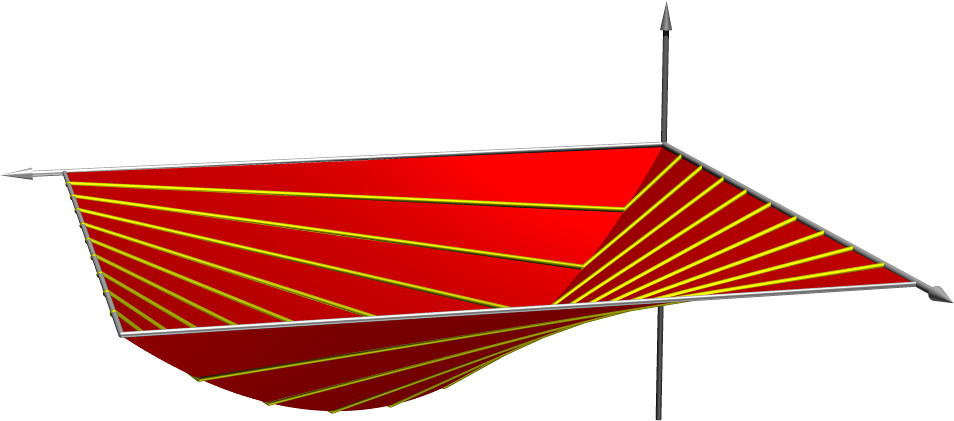
\includegraphics[width=\hsize]{../common/3d/green.jpg}
\end{center}
\caption{Graph of Green's function $G(x,\xi)$ for the problem $u''=f$ 
on the interval $[0,1]$ as a surface over the square $(x,\xi)\in[0,1]^2$.
For each value $\xi$ the partial function
$x\mapsto G(x,\xi)$ is a solution of the differential equation
$u''=\delta_\xi$ with boundary condition $u(0)=u(1)=0$.
\label{elliptisch:green3dflaeche}}
\end{figure}
\begin{figure}
\begin{center}
\includegraphics{../common/images/green-1.pdf}
\end{center}
\caption{Partial function $x\mapsto G(x,\xi)$ of Green's function
for the problem $u''=f$ with boundary conditions 
$u(0)=u(1)=0$ for various values of $\xi$.
\label{elliptisch:green1schar}}
\end{figure}

The formular for the solution $u(x)$ we have found writes the solution
as a double integral, but this is not the form we are looking for.
We want the solution as a simple integral over $[0,1]$ with integrand
$G(x,\xi) f(\xi)$.

We can use the function $h$ to fix this.
The partial function $x\mapsto h(x,\xi)=(x-\xi)\vartheta(x-\xi)$ has boundary
values $0$ and $1-\xi$, so the function
\[
G(x,\xi)
=
(x-\xi)\vartheta(x-\xi)-x(1-\xi)
=\begin{cases}
(x-\xi)+x(\xi-1)&\qquad x\le \xi \\
x(\xi-1)&\qquad x<\xi
\end{cases}
\]
has both boundary values equal to $0$.
$G$ satisfies
\[
\frac{\partial^2}{\partial x^2}G(x,\xi)=\delta(x-\xi)
\]
and
\[
G(0,\xi)=G(1,\xi)=0.
\]
A solution of the differential equation can thus be written as
\[
u(x)=\int_0^1G(x,\xi)f(\xi)\,d\xi+a(1-x)+bx.
\]

The ondimensional case shows that for the operator  $D^2$ and the
equation $D^2u=f$
we can actually find a function $G(x,\xi)$ that takes the role 
of an inverse.

Figures~\ref{elliptisch:green3dflaeche} and \ref{elliptisch:green1schar}
show Green's function $G(x,\xi)$.
The partial functions 
$x\mapsto G(x,\xi)$ are solutions of the problem
$u''=\delta_\xi$ with boundary conditions $u(0)=u(1)=0$.
In both figures, the partial functions are highlighted for 
a number of special values $\xi$.

\begin{beispiel}
The differential equation
\[
y''=\cos 3\pi x.
\]
has the solution
\[
y(x)=-\frac1{9\pi^2}(\cos 3\pi x + 2x - 1),
\]
which we can also find using Green's function:
\[
y(x)=\int_0^1 G(x,\xi)\cos 3\pi\xi\,d\xi.
\]
In figure~\ref{elliptisch:green-beispiele}
the right hand side $f(x)=\cos 3\pi x$ is approximated as a linear
combination of $\delta$-distributions (blue).
The associated solution is shown in red, it has kinks at each 
contributing $\delta$-function.
Increasing the number of $\delta$ functions produces better approximations
of the solution.
\begin{figure}
\begin{center}
\includegraphics[width=0.7\hsize]{../common/graphics/green-1.pdf}\\
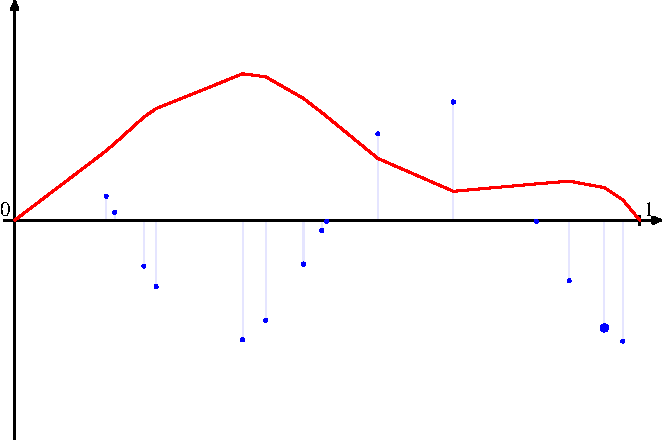
\includegraphics[width=0.7\hsize]{../common/graphics/green-324.pdf}\\
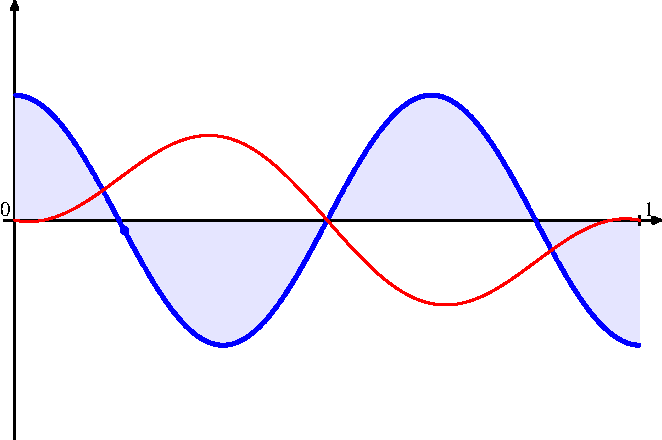
\includegraphics[width=0.7\hsize]{../common/graphics/green-1082.pdf}
\end{center}
\caption{Solution (red) of $y''=f$ and for an approximation of $f$ by
$\delta$-distributions (blue).
\label{elliptisch:green-beispiele}}
\end{figure}

An animation for the computation of $y(x)$ using Green's function
can be found on Youtube:
\url{http://www.youtube.com/watch?v=Wpi7Gf7V2HY}
\end{beispiel}

